%%Line 1810 uncomment

\documentclass[2dCFT-lecture.tex]{subfiles}


\begin{document}
\section{Renormalization group flow and \texorpdfstring{$c$}{c}-theorem}

\subsection{Renormalization group flow}

\subsubsection*{Idea}

In the introduction, we have briefly discussed that conformal field theories arise at fixed points of renormalization group flow. The study of renormalization group flows tells us the special role of conformal field theories (See \cite{Zamolodchikov:1989zs} included in \cite{jimbo2014integrable} and \cite{eguchi1989deformations}). In this section, we shall glimpse this in two-dimensional systems.


The name of renormalization group is actually misleading in the following two reasons:
\begin{itemize} \setlength{\itemsep}{-.5pt}
\item the transformations of the renormalization ``group'' are irreversible; therefore, they do not form a group. \item moreover, they do not necessarily concern the renormalization of a theory, i.e. the cure of the divergences of the perturbative series. \end{itemize}
Instead, the concept of renormalization group flow describes how families of physical theories behave under change of the length scale. The effect of averaging over short-distance physics can be summarized in the change of finitely many parameters in the long-distance physics of interest.


There is a wonderful introduction to renormalization group flow in \cite[\S3]{cardy1996scaling}. Following Cardy,
we shall explain the concept of renormalization group flow by coarse-graining for the Ising model.
Let us consider a statistical system defined on a $d$-dimensional regular lattice of spacing $a$, with degrees of freedom placed on its sites. Let $H(\{\sigma_i^{(1)}\},g_k^{(1)})$ be the Hamiltonian of the system, where $g_k^{(1)}$ are the coupling constants of the various interactions among the spins $\sigma_i^{(1)}$. Now we divide the original lattice into blocks of length $ba$, denoted by $\cB_k$, each of them made of $b^d$ spins, and we assign a new spin variable $\sigma_k^{(2)}$ by averaging over all the spins $\sigma_i^{(1)}\in \cB_k$. We are going to do coarse-graining of the original lattice by repeating this procedure. More precisely, we define the new spin variable by
\be\label{average}\sigma_{k}^{(n+1)}= A^{(n)}\sum_{i \in \mathcal{B}_{k}} \sigma_{i}^{(n)}\ee
where $A$ is a suitable normalization constant.

To define the effective hamiltonian for the coarse lattice, we introduce an operator
\[T \left(\sigma_{k}^{(n+1)}, \sigma_{i}^{(n)}\right)=\left\{\begin{array}{l}{1 ~,\quad \text{if}\ \eqref{average}}\\{0 ~,\quad \text{otherwise}} \end{array} \right.\]
so that it satisfies
\[
\sum_{\left\{\sigma_{k}^{(n+1)}\right\}}T \left(\sigma_{k}^{(n+1)}, \sigma_{i}^{(n)}\right)=1
\]
Then, the effective hamiltonian $H^{(n+1)}\left(\left\{\sigma_{k}^{(n+1)}\right\} , g_{k}^{(n+1)}\right)$ can be defined by averaging the spins $\sigma_{i}^{(n)}$ with their Boltzmann factor
\[
\exp \left[-H^{(n+1)}\left(\left\{\sigma_{k}^{(n+1)}\right\} , g_{k}^{(n+1)}\right) \right] =\sum_{\left\{\sigma_{i}^{(n)}\right\}}\prod_{\textrm{blocks}}T \left(\sigma_{k}^{(n+1)}, \sigma_{i}^{(n)}\right) \exp \left[-H^{(n)}\left(\left\{\sigma_{i}^{(n)}\right\} , g_{i}^{(n)}\right) \right]
\]
in this way. Then, ignoring an overall constant, we have the equivalence of the statistical partition functions
\[
\sum_{\left\{\sigma_{k}^{(n+1)}\right\}}\exp \left[-H^{(n+1)}\left(\left\{\sigma_{k}^{(n+1)}\right\} , g_{k}^{(n+1)}\right) \right]=\sum_{\left\{\sigma_{i}^{(n)}\right\}}\exp \left[-H^{(n)}\left(\left\{\sigma_{i}^{(n)}\right\} , g_{i}^{(n)}\right) \right]
\]
This equality also holds for the expectation value of any observable $\cO$.
In this process, the new coupling constants are expressed by the previous one
\[
\left\{g^{(n+1)}\right\}=\mathcal{R}\left(\left\{g^{(n)}\right\} \right)
\]
where $\cR$ is, in general, a complicated nonlinear transformation.Starting from the original coupling constants $\{g_k^{(1)}\}$, the procedure of the coarse-graining provides the sequence  $\{g_k^{(2)}\}$, $\{g_k^{(3)}\}$, $\ldots$, which is called a \textbf{renormalization group flow}.
 In fact, a fixed point is a point in the space of the coupling constants that remains invariant
\[
g^{*}= \mathcal{R}\left(g^{*}\right)
\]
Since the coarse-graining does not affect the theory, it is scale-invariant, implying that it is conformal.  As briefly explained in the introduction, critical phenomena are described by these fixed points.


\subsubsection*{One-dimensional Ising model}

As a concrete example, let us examine the one-dimensional Ising model whose Hamiltonian is
\[
H \left(s_{i}; J \right)=- J \sum_{i}s_{i}s_{i+1}
\]
Each pair of spins has the Boltzmann weight
\begin{equation}
  W \left(s_{i}, s_{i+1}; v \right)=e^{K s_{i}s_{i+1}}=\cosh K \left(1+v s_{i}s_{i+1}\right)
\end{equation}
where $v=\tanh K = \tanh \frac{J}{k_BT}$.

\begin{figure}[ht]\centering
\includegraphics[width=7cm]{picture/coarse-graining}\caption{coarse-graining}\label{fig:coarse-graining}
\end{figure}

As illustrated in Figure \ref{fig:coarse-graining}, we divide the lattice of three spins. Denoting $\sigma_1= s_2$ and $\sigma_2=s_5$, we sum over $s_3$ and $s_4$
\bea
\sum_{s_3,s_4}e^{J \sigma_{1}s_{3}} e^{J s_{3}s_{4}} e^{J s_{4}\sigma_{2}}&=\sum_{s_3,s_4}
(\cosh K)^{3}\left(1+v \sigma_{1}s_{3}\right) \left(1+v s_{3}s_{4}\right) \left(1+v s_{4}\sigma_{2}\right)
\cr
&=
2^{2}(\cosh K)^{3}\left(1+v^{3}\sigma_{1}\sigma_{2}\right)
\eea
In addition to a normalization constant, one can assign the new Boltzmann weight $W (\sigma_{1},\sigma_{2}; \wt v)$ to the new block spins $\sigma_{1},\sigma_{2}$ with the new coupling constant
\[
\wt v= v^{3}~,
\]
which is called the \textbf{renormalization group equation}. It has two fixed points: $v_1^*=0$ and $v_2^*=1$ corresponding to the  high-temperature phase $T\to \infty$, and the low-temperature phase $T=0$.


In addition, the new Hamiltonian of the system is  given by
\[
H \left(\sigma_{i}; \wt J\right)=\wt Np (J)-\wt J\sum_{i}\sigma_{i}\sigma_{i+1}
\]
where $\wt N=N/3$ is the number of new sites, and
\begin{equation}
\wt J  =k_BT\tanh^{- 1}\left[ (\tanh K)^{3}\right]~,\quad p (J)=- \log \left[ \frac{(\cosh K)^{3}}{\cosh \wt K} \right]-2\log 2~.
\end{equation}

\subsubsection*{$\beta$-functions and Callan-Symanzik equation}
In general, the idea described above ends up with mathematical equations describing renormalization group flows in the space of parameters of a physical system. Let us derive these equations by using path integrals. Writing the action of a conformal field theory at a fixed point by $S^*$, the perturbed action can be written as
\be\label{pertubation}
\cS=\cS^{*}+\sum_{a} \int \frac{d^2x}{2\pi}~ g_{a} \cO_{a} (x)
\ee
where the coupling constants $g_{a}$ are sufficiently small. If $\cO_{a}$ is of scaling dimension $\Delta_a$ the coupling constant $g_{a}$ has scaling dimension $2-\Delta_a$. Under an infinitesimal scaling transformation (dilatation) $x\to (1+d\lambda)x$, the perturbed action behaves as
\bea
\cS \rightarrow& \cS^{*}+\sum_{a} (1 +d\lambda)^{2} (1 +d\lambda)^{- \Delta_a} \int \frac{d^2x}{2\pi}~ g_{a} \cO_{a} (x)\cr
&\simeq \cS+d\lambda \sum_{a} \left(2-\Delta_a \right) \int \frac{d^2x}{2\pi}~ g_{a} \cO_{a} (x)
\eea
where we assume that $S^*$ is scale-invariant. On the other hand, we recall the variation under the scaling transformation
\begin{equation}
\cS \rightarrow \cS +d\lambda \int d^2x~ \left(T_{11} (x)+T_{22} (x) \right)=S - d\lambda \int \frac{d^2x}{2\pi}~  \Theta (x)\end{equation}
where
\begin{equation}\label{Theta}
  \Theta :=-2\pi{T^{\mu}}_\mu
\end{equation}
is the trace of the energy-momentum tensor. Therefore, we can write
\be\label{Theta-beta}
 \Theta (x)=-\sum_{a} \beta_{a} (g) \cO_{a} (x)
\ee
where $\beta_{a} $ are first-order approximations of so-called $\beta$-functions
\be\label{1st-approx}
\beta_{a} (g)=\left(2-\Delta_a \right) g_{a}
\ee


The idea of renormalization group flow is that the change of a physical system on the length-scale is absorbed into the change of coupling constants, which is measured by the   $\beta$-functions
\[
\frac{d g_{a}}{d\lambda}=\beta_{a} (g)
\]
Therefore, at a fixed point, we have
\[
\beta_{a} \left(g^{*} \right)=0
\]
 by definition. At the first-order approximation \eqref{1st-approx}, the coupling constants behave as
 \[
 g_{a} \sim e^{(2-\Delta_a)\lambda}
 \]
 around a fixed point $g_{a}^*=0$.

 At the long distant scale $\lambda\gg 1$ that is called \textbf{infra}-\textbf{red} or \textbf{IR},
if $\Delta_a<2$, a coupling constant increases, it is called a \textbf{relevant coupling}. If $\Delta_a>2$, it decreases and is called an \textbf{irrelevant coupling}.  In the space of coupling constants $\{g_{a}\}$, the subspace spanned by irrelevant ones is called the \textbf{critical manifold}, which is the attractive basin for the fixed point $g^*$. Under the RG flow, irrelevant operators are scaled out, and it arrives at the fixed point.
Hence, all the theories belong to the same universality class.
\begin{figure}[ht]\centering
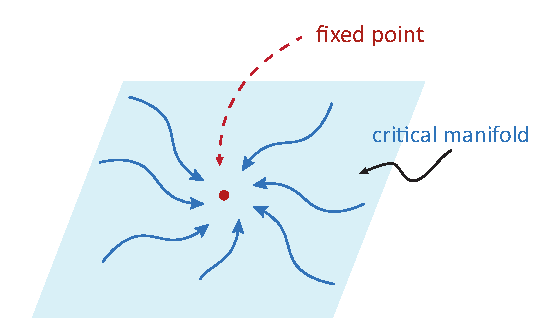
\includegraphics[width=8.5cm]{picture/critical-manifold}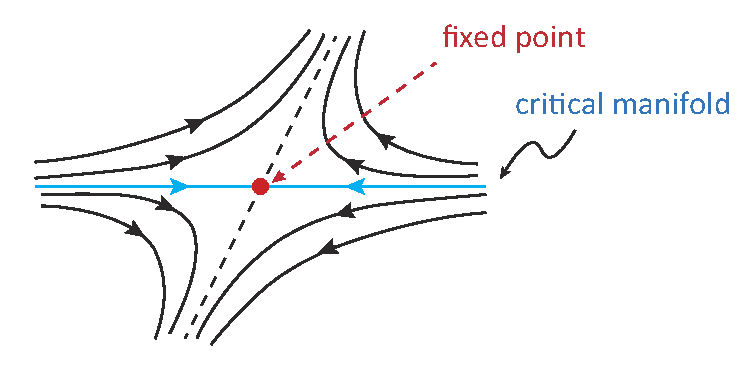
\includegraphics[width=8.5cm]{picture/RG-flow}
\end{figure}


On the other hand, the instability nature of a critical point is determined by the number of its relevant couplings. Relevant couplings get amplified as a theory flows to the low-energy region and moves away from the fixed point. When $\Delta_a=2$, an operator $\cO_{a}$ is called \textbf{marginal}, and  its behavior depends on its $\beta$-function, which is determined by taking quantum corrections into account (beyond the first-order approximation). If $\beta_{a}>0$ (resp. $\beta_{a}<0$), then it is called \textbf{marginally relevant} (resp. \textbf{marginally irrelevant}). If $\beta_{a}=0$, then it is called \textbf{exactly marginal}. Our main interest here is the two-dimensional theories, but the same argument can be applied to quantum field theories in any dimension.

Now let us consider the correlation functions of the local fields $\phi_i(x)$, defined as usual by the functional integral
\[
\left\langle \phi_{1} \left(x_{1} \right) \ldots \phi_{n} \left(x_{n} \right) \right\rangle=\int \mathcal {D} \phi ~\phi_{1} \left(x_{1} \right) \ldots \phi_{n} \left(x_{n} \right) e^{- S[ \phi ]}
\]
If the variation of the field $ \phi_{i}$ under the scaling transformation is
\[
\delta \phi_{i}(x)=-\epsilon \left(x^{\mu} \partial_{\mu}+\Delta_{i} \right) \phi_{i}(x)
\]
the corresponding Ward-Takahashi identity  \eqref{conformal-ward-identity-st} is
\be\label{WT-dilaton}
\sum_{i=1}^{n} \left\langle \left(x_i^{\mu} \frac{\partial}{\partial x_i^{\mu}}+\Delta_{i} \right) \phi_{1} \ldots \phi_{n} \right\rangle-\int \frac{d^{2} x}{2\pi} \left\langle \Theta (x) \phi_{1} \left(x_{1} \right) \ldots \phi_{n} \left(x_{n} \right) \right\rangle=0~.
\ee

The fields $\phi_i(x)$ can also depend on the coupling constants and their variation, varying the coupling $g_a$, is expressed in terms of an operator $\widehat {B}_{i}^{(a)}$
\[
\widehat {B}_{i}^{(a)} \phi_{i} (x)=\frac{\partial}{\partial g_{a}} \phi_{i} (x)
\]
Using \eqref{Theta-beta}, we can write
\begin{equation}
  \sum_{a} \beta_{a} \frac{\partial}{\partial g_{a}} \langle \phi_{1}  \ldots \phi_{n} \rangle=\sum_{i=1}^{n} \sum_{a} \beta_{a} \left\langle \widehat {B}_{i}^{(a)}\phi_{1}  \ldots \phi_{n}  \right\rangle+\int \frac{d^{2} y}{2 \pi} \langle \Theta (y) \phi_{1}  \ldots \phi_{n}  \rangle
\end{equation}
Defining the operator
\begin{equation}\label{anomalous}
  \widehat {\Gamma}_{i}= \wh\Delta_{i}+ \sum_{a} \beta_{a} \widehat {B}_{i}^{(a)}
\end{equation}
we can erase $\Theta$ from the \eqref{WT-dilaton}, which is called
the  \textbf{Callan-Symanzik equation}
\begin{equation}\label{CS-eq}
   \sum_{i=1}^{n} \left\langle \left(x_{i}^{\mu} \frac{\partial}{\partial x_{i}^{\mu}}+\widehat {\Gamma}_{i} (g) \right) \phi_{1} \left(x_{1} \right) \ldots \phi_{n} \left(x_{n} \right) \right\rangle  -\sum_{a} \beta^{a} (g) \frac{\partial}{\partial g_{a}} \left\langle \phi_{1} \left(x_{1} \right) \ldots \phi_{n} \left(x_{n} \right) \right\rangle=0~.
\end{equation}
The operator $\widehat {\Gamma}_i$ in \eqref{anomalous} determines the scaling dimension of an operator $\phi_i$ at quantum level where $\wh\Delta_i$ yields the classical scaling dimension and $\sum_{a} \beta_{a} \widehat {B}_{i}^{(a)}$ measures quantum corrections. Thus, it is called the \textbf{anomalous dimension}.
Consequently, the Callan–Symanzik equation is a differential equation describing the evolution of a correlation function under variation of the energy scale.
Since the scaling dimension of $\Theta$ is always two $\widehat {\Gamma}\Theta=2\Theta$ at quantum level, we can derive
\begin{equation}\label{anomalous2}
  \widehat {\Gamma} \cO_{a} (x)=\sum_b \gamma_{a b} \cO_b (x)=\sum_b \left(2 \delta_{a b}-\frac{\partial \beta_b}{\partial g_{a}} \right) \cO_b (x)~.
\end{equation}
Indeed, using \eqref{Theta-beta}, this form yields
\begin{equation}
\begin{aligned}
\widehat{\Gamma} \Theta &=-\left(\widehat{\Delta}+\sum_{a} \beta_{a} \frac{\partial}{\partial g_{a}}\right) \sum_{b} \beta_{b} \cO_b \\
&=-\left(\sum_{b} \beta_{b} \widehat{\Gamma} \cO_b+\sum_{a,b} \beta_{a} \frac{\partial \beta_{b}}{\partial g_{a}} \cO_b\right) \\
&=-\left(\sum_{a,b} \beta_{b}\left(2 \delta_{ba}-\frac{\partial \beta_{a}}{\partial g_{b}}\right) \cO_a+\sum_{a,b} \beta_{a} \frac{\partial \beta_{b}}{\partial g_{a}} \cO_b\right) \\
&=2 \Theta
\end{aligned}
\end{equation}
Also, in the first-order approximation \eqref{1st-approx}, it is easy to see
\[
\widehat {\Gamma} \cO_{a}=\Delta_a \cO_{a}~,
\]
as expected.












\subsection{Zamolodchikov \texorpdfstring{$c$}{c}-theorem} \label{sec:Zc}
In renormalization group flows in 2d, there is an important theorem due to A.B. Zamolodchikov, called the $c$-\textbf{theorem} \cite[ISZ88-No.45]{zamolodchikov1986irreversibility}.
The $c$-Theorem asserts that, under the assumptions of rotation
invariance, unitarity and energy-momentum conservation in a
two-dimensional theory, there exists a function $C$ which is non-increasing along a renormalization group flow. Moreover, at an IR fixed point, it is equal to
the central charge $c$ of the IR CFT. This theorem tells us the global structure of the space of physical theories and the role of conformal field theories.

We begin with energy-momentum conservation,
\begin{equation}
\partial_{\mu} T^{\mu \nu}=0\,,
\end{equation}
where $T^{\mu\nu}$ is symmetric. This can be written in complex coordinates $z$, $\overline{z}$
\begin{equation}
\label{conservation-law-Theta}
\overline\partial T+\frac{1}{4} \partial \Theta=0 \quad,\quad \partial \overline {T}+\frac{1}{4} \overline\partial \Theta=0\, ,
\end{equation}
where $\Theta :=-2\pi{T^{\mu}}_\mu$. (See \eqref{T-barT} and \eqref{holomorphic-EM}.) At an IR fixed point, $\Theta$ vanishes and $T=T(z)$ is holomorphic. However, the energy-momentum tensor is dependent of both holomorphic and anti-holomorphic coordinate $T=T(z,\overline{z})$, and $\Theta(z,\overline{z})\neq0$ for a non-conformal theory.  Since $T$, $\Theta$ and $\overline{T}$
be the components of spin $(2,0)$, $(1,1)$ and $(0,2)$, respectively, of the
energy-momentum tensor, the rotational invariance, spins and dimensions imply for the
correlation functions of $T$ and $\Theta$
\bea\label{T-Theta}
\langle T (z , \overline {z}) T (0,0) \rangle &= \frac{F (z \overline {z})}{z^{4}}\, ,\\
\langle \Theta (z , \overline {z}) T (0,0) \rangle=\langle T (z , \overline {z}) \Theta (0,0) \rangle &= \frac{G (z \overline {z})}{z^{3} \overline {z}}\,,\\
\langle \Theta (z , \overline {z}) \Theta (0,0) \rangle &= \frac{H (z \overline {z})}{z^{2} \overline {z}^{2}}\, .\,
\eea
and similarly for $\overline{T}$. Combining the
first equation of \eqref{conservation-law-Theta} with $T$, we have
\begin{equation}
\left\langle \overline\partial T (z , \overline {z}) T (0,0) \right\rangle+\frac{1}{4} \left\langle \partial \Theta (z , \overline {z}) T (0,0) \right\rangle=0\, ,
\end{equation}
We adopt the notation
$\dot {F} :=z \overline {z} F^{\prime} (z \overline {z})$ where the prime stands for the derivative of $F(x)$ with respect to its argument. One finds
\begin{equation}
\dot {F}+\frac{1}{4} \dot {G}-\frac{3}{4} G=0\, ,
\end{equation}
and similarly by combining with $\Theta$
\begin{equation}
\dot {G}-G+\frac{1}{4} \dot {H}-\frac{1}{2} H=0\, .
\end{equation}
Eliminating $G$ from above two equations,  we define
\begin{equation}\label{c-fn}
C :=2 F-G-\frac{3}{8} H\,.
\end{equation}
Then, we find that it is non-increasing with respect to the scale
\begin{equation}
\label{C-theorem}
\dot {C}=- \frac{3}{4} H \leq 0\, .
\end{equation}
due to unitarity. We see $C$ is a non-increasing function of
$R:=(z\overline{z})^{\frac12}$, for fixed values of couplings $\{g\}$.
The $R$-dependence is related to the dependence on the
$\{g\}$ via the Callan-Symanzik equation \eqref{CS-eq}
\begin{equation}
\label{callan-Symanzik equation}
\left(R \frac{\partial}{\partial R}-\sum_a \beta_a  \left(g\right) \frac{\partial}{\partial g_a} \right) C (R , \{g \})=0\, .
\end{equation}
Using \eqref{Theta-beta} and the Callan-Symanzik equation \eqref{CS-eq} on $\langle \Theta\Theta\rangle$, we obtain
\begin{equation}
\label{c{g}}
\beta^{a} \frac{\partial}{\partial g^{a}} C (g)=- \frac{3}{2} G_{a b} (g) \beta^{a} (g) \beta^{b} (g)\, ,
\end{equation}
where
\begin{equation}\label{Z-metric}
G_{a b} (g)=G_{a b} (1 , g) , \quad G_{a b} (z \overline {z} , g)=( z \overline {z})^{2} \left\langle \cO_{a} (z , \overline {z}) \cO_b (0,0) \right\rangle\, ,
\end{equation}
is positive-definite, since the theory is unitary. In other words, $G_{ab}(g)$ can be regarded as a metric of the space of the coupling constants. Therefore, it is called the \textbf{Zamolodchikov metric}. Moreover, we can write the $\beta$-function as
\be\label{grad}
\beta_{a} (g)=- \frac{2}{3}\sum_{b}G_{ab}^{- 1}\frac{\partial C}{\partial g_{b}}~,
\ee
so that $C$ can be understood as a Morse function on the space of the coupling constants and $\beta_a$ can be understood as the gradient vector fields of the Morse function \cite{milnor1963morse}.



It follows from \eqref{c{g}}  that the function $C(g)$ decreases under  the renormalization
group flow. Since the $\beta$-function vanishes at a fixed point, $C$ is stationary with respect to $R$ at the fixed point.
At the fixed point, the theory is conformal so that \eqref{T-Theta} becomes
\begin{equation}
  F=\frac{c}2~, \qquad G=0=H~.
\end{equation}
Consequently, it is equal to the central charge $C(g^*)=c$ at the fixed point $g=g^*$. This proves the statement of the
$c$-\textbf{theorem}. Consequently,  the central charge of $S$ is less than or equal to that of $S^*$ in \eqref{pertubation}
\[
c_{\textrm{UV}}\ge c_{\textrm{IR}}~.
\]
Hence, one can think that the central charge $c$ encodes degrees of freedom of the theory, and it decreases under a renormalization group flow since some massive particles are integrated out.
There is the corresponding theorem in four dimensions \cite{Komargodski:2011vj}. In six dimensions, the corresponding theorem is proven for supersymmetric theories \cite{Cordova:2015fha}.



\subsection{Landau-Ginzburg effective theory and minimal models}


\subsubsection*{Landau-Ginzburg effective theory}


Zamolodchikov has proposed \cite[ISZ88-No.17]{zamolodchikov1986conformal} that there exists a simple effective Lagrangian description for a special class of minimal models by the following action
\[\cS=\int \mathrm{d}^{2}z \left(\frac{1}{2}(\partial \Sigma)^{2}+V(\Sigma)\right)\]
where the potential
\[V (\Sigma)=g_{1}\Sigma+g_{2}\normord{\Sigma^{2}}+\cdots+g_{2 (p- 2)}\normord{\Sigma^{2 (p- 2)}}+g \normord{\Sigma^{2 (p- 1)}}\]
Note that the terms $\normord{\Sigma^{2 p-3}}$ can always be removed by a shift of the field $\Sigma\to\Sigma +$ const and absorbed in the linear term $g_1\Sigma$. Here we assume $g>0$ so that there are $(p-1)$ local minima, which corresponds to different phases of the model. This model is called \textbf{Landau-Ginzburg effective theory}.
 \begin{table}[htbp]\centering
 \begin{tabular}{c|ccccc}
		$6$
		&
		&
		&
		&
		&	\\ [5pt]
		$5$
		&
		&
		&
		&
		& $\phi_{5,5}$
		\\ [5pt]
		$4$
			&
		&
		&
		& $\phi_{4,4}$
		&$\phi_{5,4}$
		\\[5pt]
		$3$
		&
		&
		& $\phi_{3,3}$
		&$\phi_{4,3}$
     &
		\\[5pt]
			$2$
		&
			& $\phi_{2,2}$
		&$\phi_{3,2}$
		&
     &
		\\    [5pt]
				$1$
			& $1$
		&$\phi_{2,1}$
			&
		&
     &
		\\    [5pt]
		\midrule
		$0$
		& $1$
		& $2$
		& $3$	& $4$	& $5$
			\end{tabular}
\qquad
\begin{tabular}{c|ccccc}
		$6$
		&
		&
		&
		&
		&	\\ [5pt]
		$5$
		&
		&
		&
		&
		& $\Sigma^4$
		\\ [5pt]
		$4$
			&
		&
		&
		& $\Sigma^3$
		&$\Sigma^8$
		\\[5pt]
		$3$
		&
		&
		& $\Sigma^2$
		&$\Sigma^7$
     &
		\\[5pt]
			$2$
		&
			& $\Sigma$
		&$\Sigma^6$
		&
     &
		\\    [5pt]
				$1$
			& $1$
		&$\Sigma^5$
			&
		&
     &
		\\    [5pt]
		\midrule
		$0$
		& $1$
		& $2$
		& $3$	& $4$	& $5$
	\end{tabular}
	\caption{Relevant operators of conformal dimension $h < 1$ in the minimal model $\cM_6$ and the corresponding operators in the Landau-Ginzburg effective theory.}
	\end{table}

The theory consists of $2(p -2)$ scalar relevant fields, associated to the operators $\normord{\Sigma^k}$ for $1\le k\le 2(p-1)$. On the other hand, the unitary minimal model  $\cM_p$ has $2(p -2)$  primary fields  with conformal dimension $h < 1$. Hence, we identify the most relevant field $\phi_{2,2}$ of $\cM_p$ (with the lowest conformal dimension) with the scalar field $\Sigma$ in the Landau-Ginzburg theory. The OPE of $\Sigma$ is
\[
\Sigma (z) \Sigma (0)=\frac{1}{| z |^{2 h_{2,2}}}+\frac{1}{| z |^{2  h_{2,2}- h^{\prime}}}\normord{\Sigma^{2}} (0)+\cdots
\]
where $h'$ is the conformal dimension of $\normord{\Sigma^{2}}$. On the other hand,
recalling the fusion rule of primary fields \eqref{MM-fusion}
\[
\phi_{2,2}\times \phi_{r, s}= \left[ \phi_{r-1 , s-1}\right]+\left[ \phi_{r+1 , s+1}\right]+\left[ \phi_{r+1 , s-1}\right]+\left[ \phi_{r-1 , s+1}\right]~,
\]
so that
\[
\phi_{2,2}\times \phi_{2,2}= [ \mathbf{1}]+\left[ \phi_{3,3}\right]+\left[ \phi_{1,3}\right]+\left[ \phi_{3,1}\right]~.
\]
Apart from the identity operator, the conformal dimension of $\phi_{3,3}$ is lower than the other two  so that it is natural to identify
\[
\phi_{3,3}=\normord{\Sigma^2}~.
\]
The same procedure leads to
\be\label{op-corresp}\begin{array}{llll}\phi_{3,3}=\normord{\Sigma^{2}} ~,& \phi_{4,4}= \normord{\Sigma^{3}} ~,& \cdots &, \phi_{p- 1 , p- 1}= \normord{\Sigma^{p- 2}}  \\  \phi_{2,1}= \normord{\Sigma^{p- 1}} ~, & \phi_{3,2}=\normord{\Sigma^{q}} ~,&\cdots& , \phi_{p- 1 , p- 2}= \normord{\Sigma^{2 p- 4}}  \end{array}\ee
Moreover, $\normord{\Sigma^{2p-3}}$ can be obtained from the OPE of $\phi_{p-1,p-2}$ and $\phi_{2,2}$. The inversion formula \eqref{inversion-formula} identifies $\phi_{1,3}=\phi_{p-1,p-2}$ so that
\[
\phi_{2,2}\times \phi_{1,3}= \left[ \phi_{2,2}\right]+\left[ \phi_{p-2 , p-3}\right]
\]
Therefore, we can identify $\normord{\Sigma^{2p-3}}$ with the descendant $L_{-1}\overline L_{-1}\phi_{2,2}$ of $\phi_{2,2}$
\[
\normord{\Sigma^{2 p-3}}=\partial \overline{\partial} \Sigma
\]
 This is the equation of motion at the multicritical point ($g_i=0$) in Landau-Ginzburg theory.


 If $g_i=0$, the theory is invariant under $\bZ_2$ symmetry $\Sigma\to-\Sigma$ \cite[ISZ88-No.30]{Zuber:1986ng}. When $p=3$, it is the $\Sigma^4$-theory that describes the Ising model. When  $p=4$, it is the $\Sigma^6$-theory that describes the tricritical Ising model. For a generic positive integer $p$, it describes the RSOS model \cite[ISZ88-No.31]{Andrews:1984af}.

The correspondence between the minimal models and the Landau-Ginzburg models can also be seen even with $\cN=2$ superconformal symmetry.  This is related to the ADE classification studied in \S\ref{sec:su2k-character}, which admits a profound interpretation in geometry.

\subsubsection*{Minimal Models and Renormalization Group Flows}

In fact, the minimal models provide a perfect platform to understand renormalization group flows \cite{Zamolodchikov:1987ti}. Let us consider the perturbation of the unitary minimal model $\cM_p$ by the primary field $\phi_{1,3}$
\[\cS=\cS_ {p} + g \int \frac{d^{2} x}{2\pi} \phi_{1,3} ( x )~\]
where we assume $p\gg1$. Then, the primary field $\phi_{1,3}$ can be considered as a quasi-marginal operator since the scaling dimension is
\[\Delta_{1,3}  = 2 h_{1,3} = 2 - \frac{4}{p + 1} \equiv 2 - \epsilon\]
with $\e\ll1$.
Following the fusion rule  \eqref{MM-fusion}, one can read off
\[\phi_{1,3} \times \phi_{1,3} = 1 + \mathbf {C}_{1} \phi_{1,3} + \mathbf {C}_{2} \phi_{1,5}~.\]
Since $ \phi_{1,5}$ is an irrelevant operator, the operator expansion above implies the renormalization of the field  $\phi_{1,3}$, which does not mix with any other fields. In fact, the structure constant is computed in \cite[ISZ88-No.15]{Dotsenko:1984nm}
\[
\begin{aligned} \mathbf {C}_{1} & = \frac{4}{\sqrt {3}} \frac{( 1 - \epsilon )^{2}}{( 1 - \epsilon / 2 ) ( 1 - 3 \epsilon / 4 )} \left[ \frac{\Gamma ( 1 - \epsilon / 4 )}{\Gamma ( 1 + \epsilon / 4 )} \right]^{\frac{3}{2}} \left[ \frac{\Gamma ( 1 + 3 \epsilon / 4 )}{\Gamma ( 1 - 3 \epsilon / 4 )} \right]^{\frac{1}{2}}  \left[ \frac{\Gamma ( 1 + \epsilon / 2 )}{\Gamma ( 1 - \epsilon / 2 )} \right]^{2} \frac{\Gamma ( 1 - \epsilon )}{\Gamma ( 1 + \epsilon )} \\ & = \frac{4}{\sqrt {3}} \left( 1 - \frac{3 \epsilon}{4} + O \left( \epsilon^{2} \right) \right) \end{aligned}
\]
In Homework 8, we have seen that the $\b$-function can be written as
\[
\frac{d g }{d \lambda} \equiv \beta  ( g ) = \epsilon g - \frac{ \mathbf {C}_{1}}{2}g^{2} +\cO(g^3)~.
\]
Using the gradient flow equation \eqref{grad}, one obtains
\[
C(g)=c_p+\a \left[\frac\epsilon2 g^{2} -\frac{ \mathbf {C}_{1}}{6}g^{3}\right] +\cO(g^4)
\]
where $c_p$ is the central charge \eqref{c<1-unitary-c} of $\cM_p$. Note that $\a$ depends on the Zamolodchikov metric $G_{ab}$ in \eqref{Z-metric}, and $\a$ can be evaluated as follows. The difference between the central charges at UV and IR can be computed by \eqref{C-theorem}
\[
\Delta c = -\frac{3}{4} \int_{0}^{\infty} d ( r^{2} ) r^{2} \langle \Theta ( r ) \Theta ( 0 ) \rangle
\]
Furthermore, \eqref{Theta-beta} tells us that
\bea
\Delta c &= -\frac{3}{4}(\e g)^2 \int_{0}^{\infty} d ( r^{2} ) r^{2} \langle \phi_{1,3} ( r ) \phi_{1,3} ( 0 ) \rangle\cr
&= -\frac{3}{2}(\e g)^2\int_{0}^{\infty} \frac{r^{3}dr}{r^{2 \Delta_{1,3}}}\cr
&=-\frac{3}{4} \e g^2 +\cO({\e^0})~.
\eea
Therefore, we have $\a=-\frac{3}{2}$. At the fixed point $g^{*} =2 \epsilon /\mathbf {C}_{1}$, the Zamolodchikov $C$-function is
\bea
C(g^*)&=c_p- \frac{ \epsilon^{3}}{ \mathbf {C}_{1}^{2}}+\mathcal {O} \left( \epsilon^{4} \right)\cr
& = c_{p} - \frac{3}{4^{2}} \cdot \left( \frac{4}{p} \right)^{3} + \cO \left( p^{- 4} \right) \\ & = c_{p} - \frac{12}{p^{3}} + \cO \left( p^{- 4} \right) \sim c_{p - 1} \eea
At this perturbative order, the new value of the central charge coincides with that of the unitary minimal model $\cM_{p-1}$. Therefore, the perturbation by $\phi_{1,3}$ leads to the renormalization group flow from $\cM_p$ to $\cM_{p-1}$.
Although we have assumed $p\gg1$ in this analysis, the evidence of RG flow from $\cM_p$ to $\cM_{p-1}$ for an arbitrary $p$ has been shown by using factorized $S$-matrices \cite{Zamolodchikov:1991vh}. In fact, from \eqref{anomalous2}, one can deduce the conformal dimension of the operator $\phi_{1,3}$ at the fixed point
\[
2 - \frac { \partial \beta  } { \partial g  }\Big|_{g=g^*}=2+\e+\cO(\e^2)~,
\]
which can be read off as the conformal dimension of $\phi_{3,1}$ in $\cM_{p-1}$ at the fixed point. Thus, the relevant operator at UV becomes the irrelevant operator at IR. (See Figure \ref{fig:rg-minimal-model}.)

\begin{figure}
	\centering
	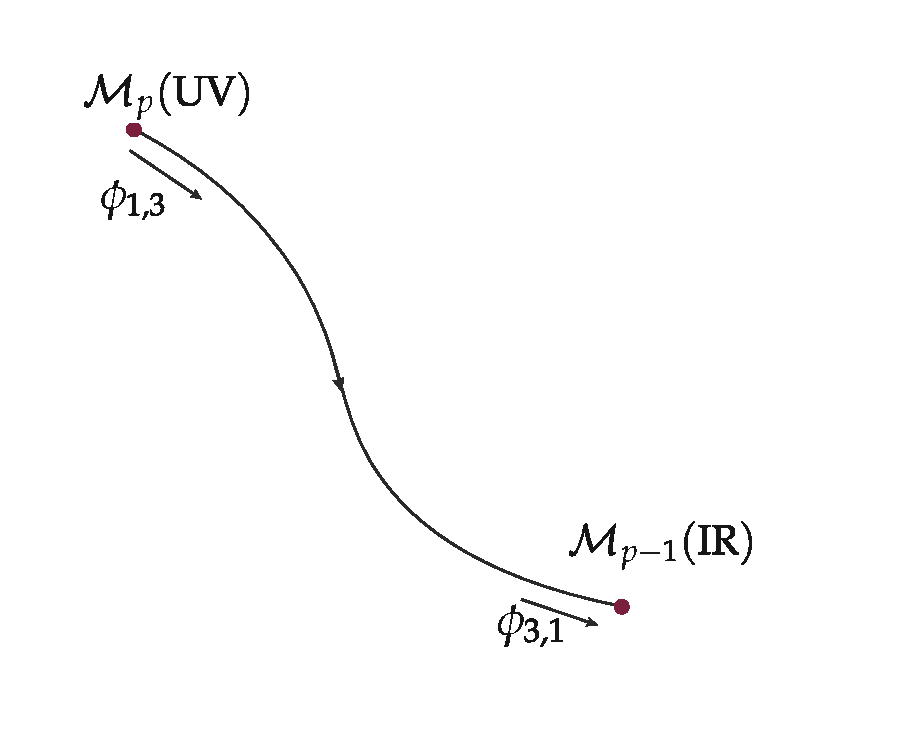
\includegraphics[width=0.5\linewidth]{picture/RG-Minimal-model}
	\caption{RG-flow between minimal models}
	\label{fig:rg-minimal-model}
\end{figure}


In fact, this is consistent with the Landau-Ginzburg effective theory. As we have seen in \eqref{op-corresp}, $\phi_{1,3} = \phi_{p - 1 , p - 2} \sim \normord{\Sigma^{2p-4}}$. Hence, the  Landau-Ginzburg action for  $\cM_{p}$ with the perturbation is
\[\cS=\int \mathrm{d}^{2}z \left(\frac{1}{2}(\partial \Sigma)^{2}+g_{2p-4}\Sigma^{2p-4}+g_{2p-2}\Sigma^{2p-2}\right)~.\]
Then, the operator $\normord{\Sigma^{2p-2}}$ becomes irrelevant and the effective action is
\[\cS=\int \mathrm{d}^{2}z \left(\frac{1}{2}(\partial \Sigma)^{2}+g_{2p-4}\Sigma^{2p-4}\right)~,\]
which is the effective action for $\cM_{p-1}$.






\end{document}
